\section{Summary}\label{sec:ciConclusion}

A search for new physics in non-resonant dilepton production via the dielectron and dimuon invariant-mass spectra has been presented.
This search made use of the full 139 fb$^{-1}$ of proton--proton collision data collected by ATLAS during Run~2 of the LHC at $\sqrt{s}=13$~TeV.
No significant excess in the collected data is observed above the expected background.
Upper limits are set on the \xsbr of new signal processes and lower limits on the CI scale \lam.
The limits on \xsbr are easily reinterpreted in terms of new physics models.
This is the first time such results have been made available.
\footnote{Precise values for the limits are publicly accessible: \url{https://www.hepdata.net/record/ins1802523}.}
The limits on \lam are the most robust frequentist limits ever set on contact interaction models.

\begin{figure}[htb]
\centering
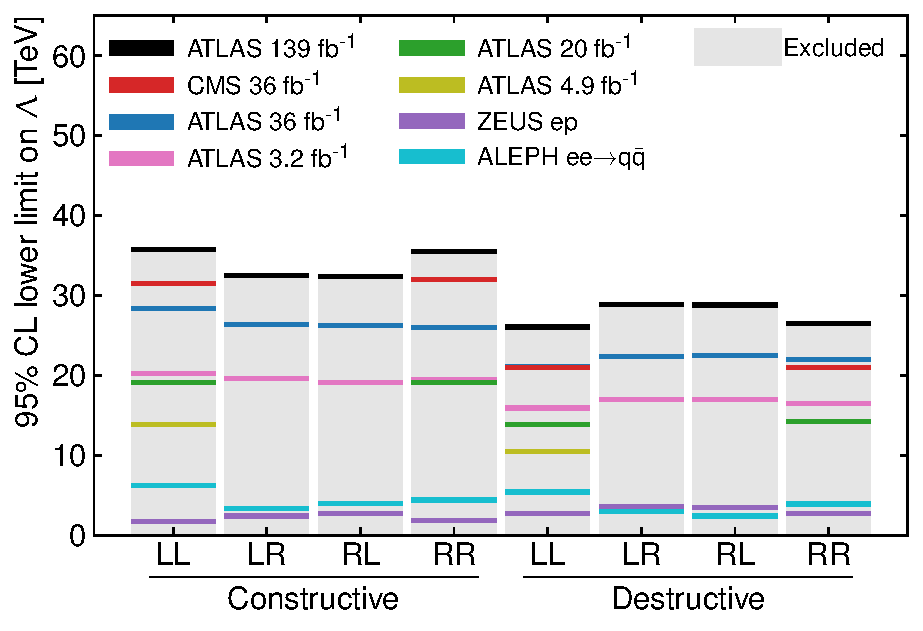
\includegraphics[width=0.70\textwidth]{figures/ci/results/hist-lambda-ll-Lambda.pdf}
\caption{
Comparison the new observed limits on \lam, shown in black, with similar \ll observations by ATLAS and other experiments.
The ATLAS results listed use datasets $\sqrt{s}=13$~TeV 36.1 fb$^{-1}$ \cite{EXOT-2016-05}, $\sqrt{s}=13$~TeV 3.1 fb$^{-1}$ \cite{EXOT-2015-07}, $\sqrt{s}=8$~TeV 20 fb$^{-1}$ \cite{EXOT-2013-19}, and $\sqrt{s}=7$~TeV 5.0 fb$^{-1}$ \cite{EXOT-2012-17}.
The most recent CMS result $\sqrt{s}=13$~TeV 36 fb$^{-1}$ is shown in red \cite{cmsCi}.
Several older studies set limits on combined LR+RL chirality models, which are not comparable to those set in this work.
The older ZEUS \cite{zeusCi} and ALEPH \cite{alephCi} results appear at the bottom.
}
\label{fig:ciHistoricalLimits}
\end{figure}

% Improvements
A number of new techniques were developed in order to enable the production of this result.
% Data driven
Most significantly, the results make use of a background estimate derived from the data in a low mass control region.
This approach replaces theoretical and experimental uncertainties with well studied statistical uncertainties on the background estimate.
These uncertainties are measured directly and robustly.
In particular, a new method for measuring spurious signal has been introduced with the ISS procedure.
% Frequentest
Additionally, the limits on both \xsbr and \lam are set using a frequentist approach.
This eliminates arbitrary prior probabilities on signal models.
These techniques, along with the integrated luminosity of the full Run~2 dataset, allow this search to probe unprecedented energy and length scales.
The strongest limits are set on the combined left-left chirality constructive model.
These observed (expected) limits exclude this model for \lam up to 35.8 (27.6)~TeV at 95\% CL.


The results of this analysis are placed in a broader context with other studies in Figure \ref{fig:ciHistoricalLimits}.
This plot shows the most recent observed limits along with earlier results by the ATLAS, CMS, ZEUS, and ALEPH collaborations from the past two decades.
The new limits on \lam use new techniques and statistical interpretation to replicate prior exclusions.
The excluded region, illustrated by the shaded grey region, has been expanded and pushes the limit on \lam higher than any previous comparable limit.




